\chapter{ตัวแบบแถวคอย (Queuing Theory)}

\section{บทนำ}
\begin{itemize}
	\item ระบบแถวคอย (การเข้าคิว) คือระบบที่มีผู้ให้บริการและมีผู้มารับบริการ โดยที่ผู้รับบริการอาจจะได้รับบริการทันที หรืออาจจะต้องรอเพื่อรับบริการตามลำดับ
	\item เป้าหมายของบทนี้คือวิเคราะห์และอธิบายระบบการเข้าแถวแบบต่าง ๆ ในแง่ของต้นทุนและแรงงาน
\end{itemize}

\section{โครงสร้างของระบบแถวคอย}
โครงสร้างสำคัญของระบบแถวคอยประกอบด้วย
\begin{enumerate}
	\item ลูกค้า (ผู้มาใช้บริการ): ลักษณะการมาเป็นอย่างไร (อัตราการมา)
	\item รูปแบบของระบบบริการ: มีกี่แถว มีกี่หน่วยบริการ และกระบวนต่อจากการให้บริการของหน่วยบริการเป็นอย่างไร
	\item หน่วยให้บริการ: อัตราการให้บริการเป็นอย่างไร
\end{enumerate}
\begin{figure}[h]
	\centering
	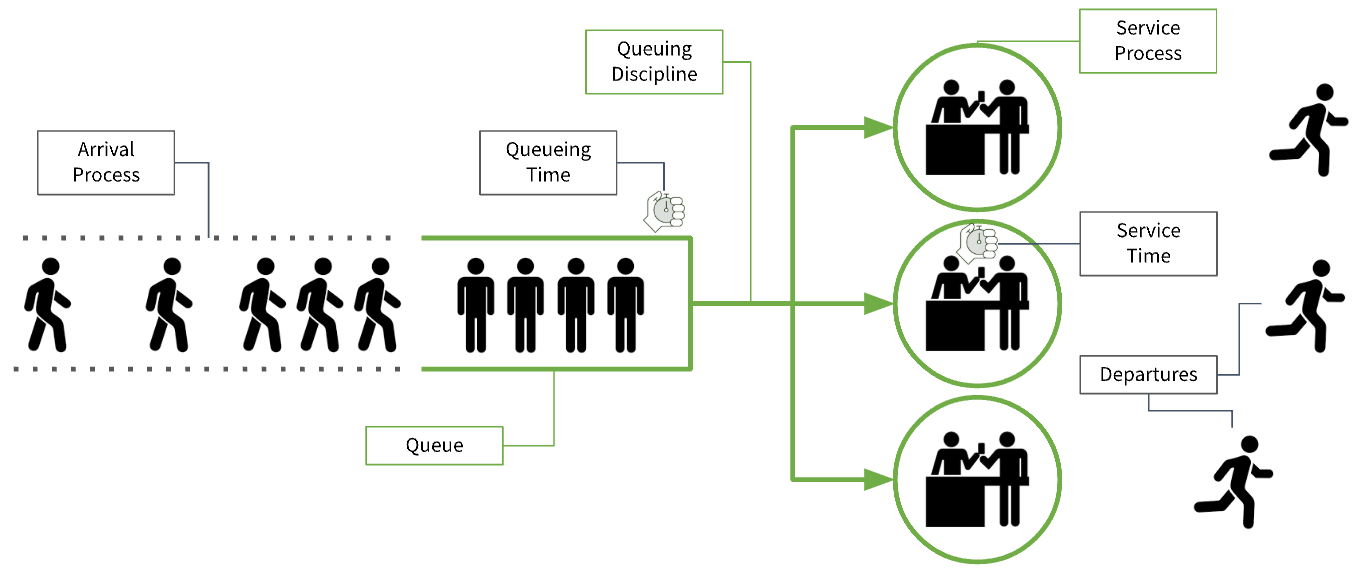
\includegraphics[width=1\linewidth]{image/queue}
\end{figure}

\subsection{ลักษณะของลูกค้า}
จำนวนผู้เข้ารับบริการ:
\begin{itemize}
	\item มีผู้เข้ารับบริการได้ไม่จำกัด
	\item มีผู้เข้ารับบริการได้จำกัด
\end{itemize}

นอกจากประเดินเรื่องความจำกัดของผู้เข้าคิวแล้ว ยังมีประเด็นเรื่องอัตราการมาเข้ารับบริการ (arrival rate) ซึ่งมักสมมติเป็น 2 รูปแบบ
\begin{itemize}
	\item ผู้เข้ารับบริการมาแบบอัตราคงที่
	\item ผู้เข้ารับบริการมาแบบสุ่ม ซึ่ง\underline{มัก}ถูกสมมติให้สุ่มด้วยการแจกแจงแบบปัวซง (Poisson distribution) 
\end{itemize}
ทั้งนี้การแจกแจงความน่าจะเป็นของการมาเข้ารับบริการอาจจะมีการแจกแจงแบบอื่นได้เช่นกันขึ้นอยู่กับสภาพแวดล้อมของแต่ละธุรกิจ

\subsubsection*{Arrival Rate: Poisson distribution}
\begin{property}
	{การแจกแจงปัวซงของอัตราการเข้ารับบริการ}{}
	กำหนดให้ $X$ เป็นตัวแปรสุ่มแทนจำนวนผู้เข้ารับบริการในช่วงระยะเวลาที่กำหนด เราจะกำหนดให้ $X$ มีการแจกแจงแบบปัวซงที่อัตราเฉลี่ยของการเข้ารับบริการมีค่าเท่ากับ $\lambda$ กล่าวคือ ความน่าจะเป็นที่จะมีผู้เข้าใช้บริการ $x$ คนมีค่าเท่ากับ
	$$
	P(X = x) = \frac{e^{-\lambda}\lambda^x}{x!}
	$$
\end{property}
\begin{example}
	{Warm-up Poisson}{}
	ในการทำการสำรวจอัตราการเข้าใช้บริการ ณ ร้านค้าแห่งหนึ่งในช่วงระยะเวลา 1 ชั่วโมง ผู้สำรวจพบว่าค่าเฉลี่ยการมาเข้าใช้บริการของบุคคลทั่วไปคือ 10 คน ต่อชั่วโมง กำหนดให้จำนวนผู้ใช้บริการห้างสรรพสินค้าแห่งนี้มีการแจกแจงแบบปัวซง จงหาความน่าจะเป็นต่อไปนี้
	\begin{enumerate}
		\item ความน่าจะเป็นที่จะมีผู้เข้าใช้บริการ 15 คน
		\item ความน่าจะเป็นที่จะมีผู้เข้าใช้บริการไม่เกิน 5 คน
		\item ความน่าจะเป็นที่จะมีผู้เข้าใช้บริการเกิน 5 คน
	\end{enumerate}
\end{example}
\newpage
\subsubsection*{Arrival Time Interval: Exponential distribution}
นอกจากการแจกแจงความน่าจะเป็นของจำนวนผู้เข้าใช้บริการที่มีการแจกแจงแบบปัวซงแล้วนั้น ยังมีการแจกแจงอีกแบบที่มีความสัมพันธ์เกี่ยวข้อกันคือการแจกแจงความน่าจะเป็นของระยะห่างเวลาระหว่างการเข้ามารับบริการ (arrival time interval)
\begin{property}
	{การแจกแจงเอกซ์โพเนเชียลของระยะห่างเวลาระหว่างการเข้ามารับบริการ}{}
	กำหนดให้ $X$ เป็นตัวแปรสุ่มแทนระยะห่างเวลาระหว่างการเข้ามารับบริการ เราจะกำหนดให้ $X$ มีการแจกแจงแบบเอกซ์โพเนนเชียลที่...
%	อัตราเฉลี่ยของการเข้ารับบริการมีค่าเท่ากับ $\lambda$ กล่าวคือ ความน่าจะเป็นที่จะมีผู้เข้าใช้บริการ $x$ คนมีค่าเท่ากับ
%	$$
%	P(X = x) = \frac{e^{-\lambda}\lambda^x}{x!}
%	$$
\end{property}

\subsection{ลักษณะของแถวคอย}
\subsection{ลักษณะของหน่วยให้บริการ}


\section{ตัวแบบแถวคอย}
\subsection{ตัวแบบ M/M/1}
\subsection{ตัวแบบ M/M/s}
\subsection{ตัวแบบ M/G/1}
\subsection{ตัวแบบ M/D/1}

\section{การวิเคราะห์ระบบแถวคอยเพื่อการตัดสินใจทางธุรกิจ}
\subsection{การกำหนดจำนวนหน่วยบริการ}
\subsection{การตัดสินใจจัดรูปแบบแถวคอย}